% Chapitre 2 - Page 8 | Travaux Avant-Projet | L3 ELN
\documentclass[11pt,a4paper]{article}
\usepackage{fontspec}
\setmainfont{TeXGyrePagella}
\usepackage[french]{babel}
\usepackage{graphicx,tikz,xcolor,geometry}
\usetikzlibrary{calc}
\geometry{margin=0pt}
\pagestyle{empty}
\definecolor{bleufonce}{HTML}{1B3A6B}
\definecolor{bleupale}{HTML}{D9E9FB}
\definecolor{bleugris}{HTML}{5C7190}
\newcommand{\pos}[4]{\node[anchor=north west,inner sep=0pt,outer sep=0pt,text width=#3,align=left] at ($(current page.north west)+(#1,-#2)$) {#4};}
\newcommand{\sect}[1]{{\color{bleufonce}\bfseries\fontsize{17}{19}\selectfont #1}}
\newcommand{\step}[1]{{\color{bleufonce}\bfseries\fontsize{12.5}{14.5}\selectfont #1}}
\newcommand{\smallfont}{\fontsize{9.5}{11.7}\selectfont}
\newcommand{\legende}[1]{{\color{bleugris}\fontsize{8.5}{10}\selectfont #1}}
\newcommand{\puce}{\textcolor{bleufonce}{\textbullet}\enspace}
\newcommand{\marque}[2]{\node[circle,fill=bleufonce,draw=white,line width=.6pt,text=white,inner sep=0pt,minimum size=5.4mm,font=\bfseries\fontsize{9}{9}\selectfont] at #1 {#2};}
% \shot{x}{y}{largeur}{hauteur}{fichier} : capture encadrée
\newcommand{\shot}[5]{\node[anchor=north west,inner sep=0pt,outer sep=0pt] at ($(current page.north west)+(#1,-#2)$) {\includegraphics[width=#3]{#5}};
  \draw[bleufonce!75,line width=.55pt,rounded corners=1mm]
    ($(current page.north west)+(#1,-#2)+(-.4mm,.4mm)$) rectangle ($(current page.north west)+(#1,-#2)+(#3,-#4)+(.4mm,-.4mm)$);}
\begin{document}
\begin{tikzpicture}[remember picture,overlay]
\draw[bleufonce,line width=.95pt,rounded corners=8mm]
 ($(current page.north west)+(5mm,-5mm)$) rectangle ($(current page.south east)+(-5mm,5mm)$);

\pos{10mm}{13mm}{189mm}{\sect{6. Notre exemple sous Tinkercad}}
\pos{10mm}{25mm}{188mm}{{\fontsize{10.5}{13}\selectfont L'exemple utilise une \textbf{photorésistance} (LDR) reliée à l'entrée \textbf{A0} et une \textbf{LED} reliée à la broche \textbf{9} : la luminosité de la LED suit la lumière mesurée.}}

% --- Étape 4 ---------------------------------------------------------------------
\pos{10mm}{38mm}{188mm}{\step{Étape 4 --- Ajouter les composants}}
\shot{14mm}{47mm}{74mm}{47.9mm}{assets/T06_recherche.png}
\pos{95mm}{48mm}{102mm}{{\smallfont
  \puce Dans le panneau \textbf{Composants}, choisir la liste \textbf{Tout}.\\[1.3mm]
  \puce Taper le nom du composant, de préférence en anglais (\emph{photoresistor}, \emph{LED}, \emph{resistor}\ldots).\\[1.3mm]
  \puce \textbf{Glisser} le composant sur le plan de travail.\\[1.3mm]
  \puce Un \textbf{clic} sur un composant placé ouvre ses propriétés (valeur d'une résistance, couleur d'une LED\ldots).\\[1.3mm]
  \puce Pour tracer un fil : cliquer sur une broche, puis sur la broche d'arrivée.}}
\pos{14mm}{97mm}{184mm}{\legende{Figure 9 --- Recherche de la photorésistance dans la liste \textbf{Tout}.}}

% --- Étape 5 ---------------------------------------------------------------------
\pos{10mm}{107mm}{188mm}{\step{Étape 5 --- Programmer et simuler}}
\begin{scope}[shift={($(current page.north west)+(13mm,-116mm)$)},x=1mm,y=-1mm]
  \node[anchor=north west,inner sep=0pt] at (0,0) {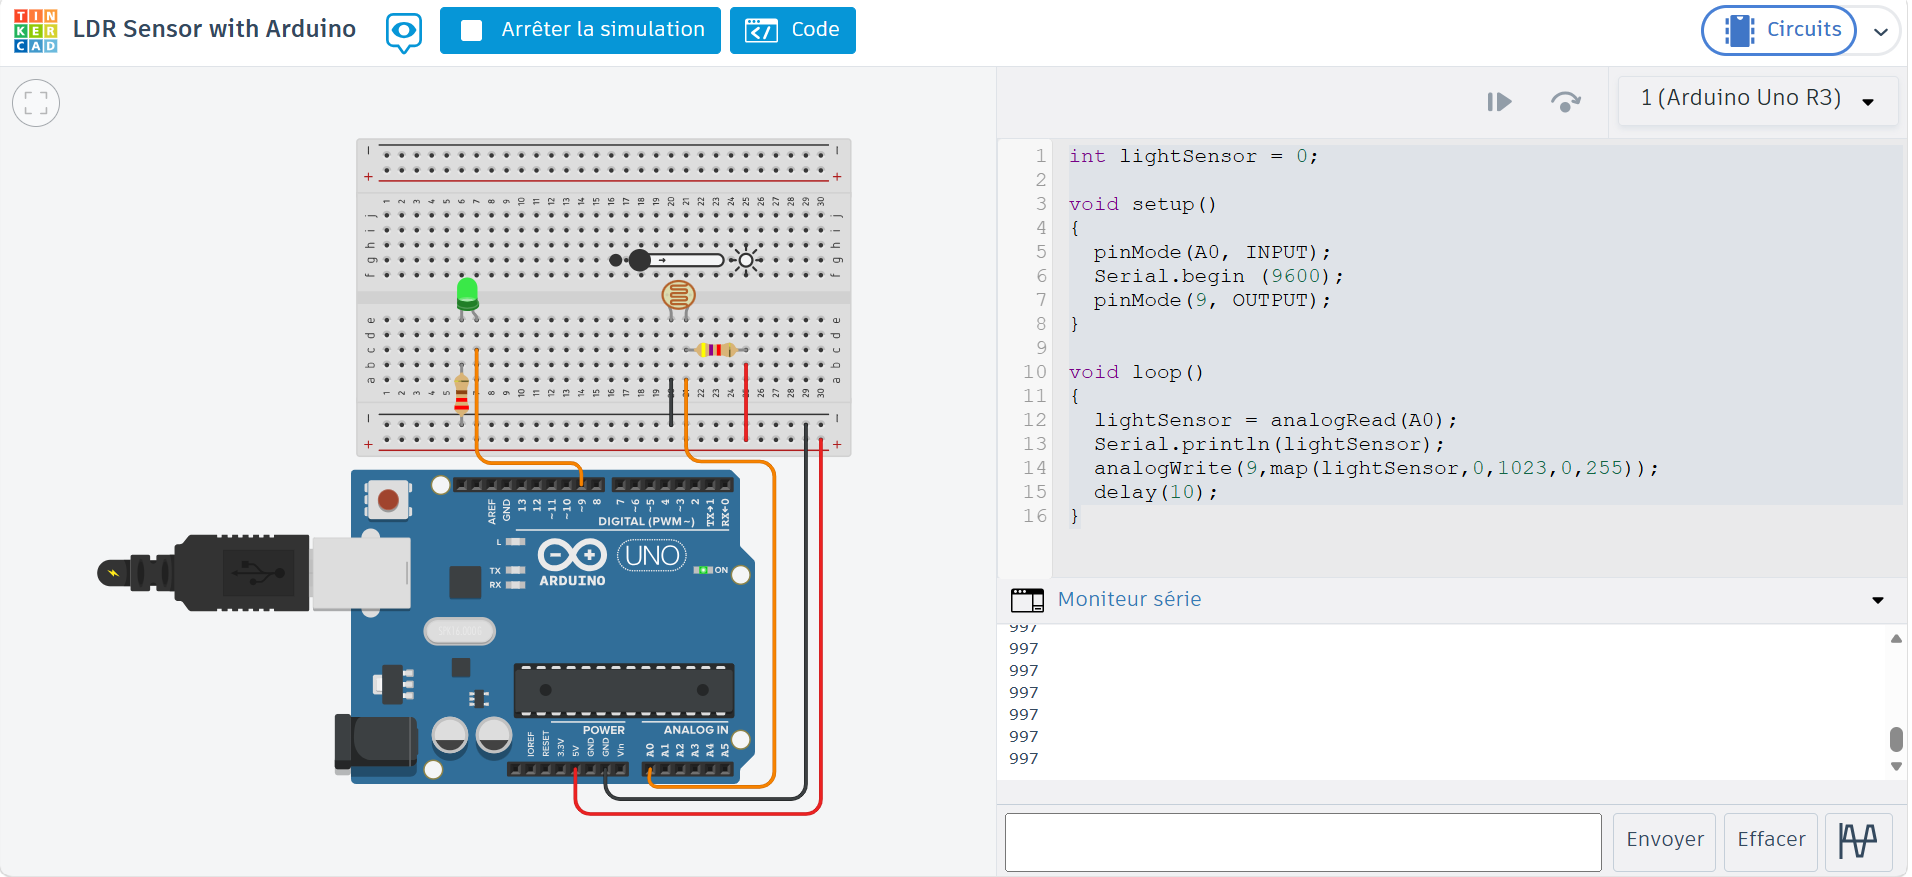
\includegraphics[width=184mm]{assets/T07_simulation.png}};
  \draw[bleufonce!75,line width=.55pt,rounded corners=1mm] (-.4,-.4) rectangle (184.4,84.8);
  % 1 px de la capture = 184/1912 mm
  \marque{(41,2.9)}{1}
  \marque{(84,2.9)}{2}
  \marque{(75,23)}{3}
  \marque{(41.5,27)}{4}
  \marque{(156,41)}{5}
  \marque{(123.5,57.6)}{6}
\end{scope}
\pos{13mm}{204mm}{186mm}{\legende{Figure 10 --- Simulation de l'exemple : montage, programme et moniteur série.}}

\pos{14mm}{212mm}{88mm}{{\smallfont \textcolor{bleufonce}{\textbf{1. Démarrer / Arrêter la simulation}} : lance ou arrête le circuit.}}
\pos{108mm}{212mm}{90mm}{{\smallfont \textcolor{bleufonce}{\textbf{2. Code}} : ouvre l'éditeur ; choisir le mode \textbf{Texte} pour écrire le programme Arduino.}}
\pos{14mm}{223mm}{88mm}{{\smallfont \textcolor{bleufonce}{\textbf{3. Curseur de lumière}} : pendant la simulation, un clic sur la LDR permet de faire varier la lumière.}}
\pos{108mm}{223mm}{90mm}{{\smallfont \textcolor{bleufonce}{\textbf{4. LED}} (broche 9, PWM) : sa luminosité suit la valeur lue sur A0.}}
\pos{14mm}{234mm}{88mm}{{\smallfont \textcolor{bleufonce}{\textbf{5. Programme}} : \texttt{analogRead(A0)} donne 0 à 1023, \texttt{map()} convertit en 0 à 255, \texttt{analogWrite(9, \ldots)} commande la LED.}}
\pos{108mm}{234mm}{90mm}{{\smallfont \textcolor{bleufonce}{\textbf{6. Moniteur série}} : affiche les valeurs envoyées par \texttt{Serial.println()} (ici 997 : forte lumière).}}

% --- À vous de jouer -------------------------------------------------------------
\fill[bleupale!55,rounded corners=2mm]
  ($(current page.north west)+(11mm,-251mm)$) rectangle
  ($(current page.north west)+(199mm,-267mm)$);
\pos{16mm}{254mm}{178mm}{{\fontsize{9.4}{11.4}\selectfont \textcolor{bleufonce}{\bfseries À vous de jouer :} transformer cet exemple en \textbf{lampe automatique} : modifier le programme pour que la LED s'allume davantage quand la lumière \textbf{diminue} (indice : inverser les deux dernières bornes de la fonction \texttt{map()}).}}

\draw[bleufonce!55,line width=.45pt] ($(current page.south west)+(10mm,14.7mm)$)--($(current page.south east)+(-10mm,14.7mm)$);
\node[anchor=south west,inner sep=0pt,text=bleufonce!80] at ($(current page.south west)+(10mm,7.4mm)$) {\fontsize{9.5}{11}\selectfont 2026/2027};
\node[anchor=south east,inner sep=0pt,text=bleufonce!80] at ($(current page.south east)+(-10mm,7.4mm)$) {\fontsize{9.5}{11}\selectfont Page 8};
\end{tikzpicture}
\null
\end{document}
